\documentclass{standalone}
\usepackage{tikz}
\begin{document}
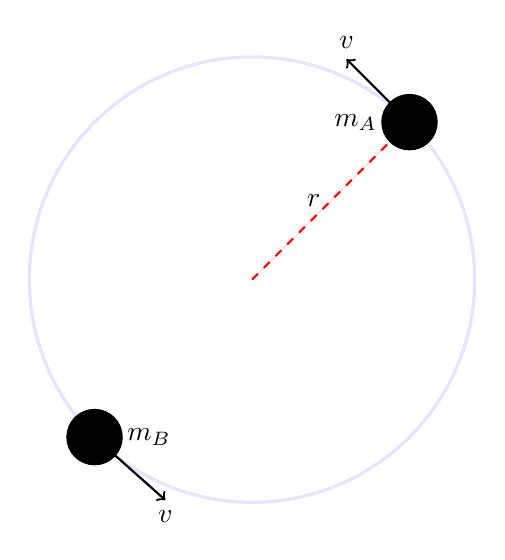
\begin{tikzpicture}
    \draw[color=blue!10, very thick](0,0) circle (2.828);
    \filldraw[red, dashed, thick] ( 0, 0) -- (2, 2) node[midway,left] {\textcolor{black}{$r$}};
    \filldraw[black] ( 2, 2) circle (10pt) node[left] { $m_A\;\;\;$};
    \draw[thick, ->] ( 2, 2) -- ( 1.2, 2.8) node[above] {$v$};
    \filldraw[black] (-2,-2) circle (10pt) node[right] { $\;\;\;m_B$};
    \draw[thick, ->] (-2,-2) -- (-1.1,-2.8) node[below] {$v$};
    %\node[] at (0,-2) {$\left(\frac{v}{c}\right)^2 \ll 1$};
    \end{tikzpicture}
\end{document}
